Um padrão tem quatro elementos essenciais:
\begin{enumerate}
\item O \emph{nome do padrão} permite distinguir rapidamente o padrão de outros e ter uma noção da aplicação e o que é o padrão. Encontrar bons nomes pode ser difícil, mas provavelmente podemos aplicar também a regra da coesão aqui: Se não há uma boa maneira de nomeá-lo, há uma boa chance do padrão não está correto. Óbvio existem exceções para esta regra e, às vezes, precisamos criar um nome novo (uma palavra nova) para representar o conceito.

\item O \emph{problema} descreve quando aplicar o padrão. Ele explica o problema e seu contexto (as forças relevantes).

\item A \emph{solução} descreve os elementos que compõe o projeto, seus relacionamentos, responsabilidades e colaborações. A solução não descreve um projeto concreto específico, ou uma implementação.

\item As \emph{consequências} descrevem os resultados e as limitações de  aplicar o padrão. As consequências para software em geral se preocupam com as limitações de tempo de execução e espaço de memória. Elas também podem tratar de problemas com a linguagem de programação e a implementação. As consequências de um padrão incluem aspectos do impacto sobre a flexibilidade do sistema, extensibilidade e portabilidade da solução.

\end{enumerate}

\cite{design:patterns} classifica os padrões de projetos do ponto de vista do propósito em três categorias:
\begin{enumerate}
\item \textbf{Criação: } Padrões de criação lidam com a criação de objetos.

\item \textbf{Estrutura: } Padrões de estrutura lidam com a composição de classes e objetos.

\item \textbf{Comportamento: } Padrões de comportamento caracterizam as maneiras como as classes e objetos interagem e distribuem responsabilidade.

\end{enumerate}

Os padrões também podem ser classificados de acordo com o escopo de aplicação do padrão: Se o padrão se aplica sobre as classes ou sobre os objetos. Padrões de classes lidam com os relacionamentos entre as classes e suas subclasses. Estes relacionamentos são estabelecidos através de herança, portanto são estáticos, fixados durante a compilação. Os padrões de objetos lidam com o relacionamento entre os objetos, que podem mudar durante a execução, portanto são mais dinâmicos.

As oito características básicas na descrição dos padrões de acordo com \citeonline{design:patterns} são:
\begin{description}
\item[Nome:] Todos os padrões devem ter um único nome que os identifica.

\item[Propósito:] O propósito do padrão.

\item[Problema:] O problema que o padrão tenta resolver.

\item[Solução:] Como o padrão fornece uma solução ao problema no contexto em que ele se encaixa.

\item[Participantes e Colaboradores:] As entidades envolvidas no padrão.

\item[Consequências:] As consequências de usar o padrão. Investiga as forças relevantes no emprego do padrão.

\item[Implementação:] Como o padrão pode ser implementado. Observação: Implementações são manifestações concretas de padrões, não devem ser entendidas como o padrão em si.

\item[Estrutura Genérica:] Um diagrama UML que mostra a estrutura típica do padrão.

\end{description}

\section{Catálogo de Padrões}

Começaremos apresentando um catálogo de padrões de projetos dos dois livros, \cite{design:patterns} e \cite{DP:explained}. Durante a exposição dos padrões, veremos algumas aplicações deles. Em geral, não aplicamos os padrões de maneira isolada, mas, para resolver problemas práticos, aplicamos diversos padrões. Apesar da \textit{gang de 4}\footnote{\cite{design:patterns}} apresentar os padrões em ordem alfabética, procuraremos estudar os padrões pelos mais simples e familiares. Já apresentamos o padrão Singleton no capítulo anterior, página \pageref{p:singleton}. Além disso, procuramos deixar próximos os padrões que estão correlacionados.

\subsection{O Padrão Fachada (\textit{Facade})}
\subsubsection{Propósito}
Fornece uma interface unificada para um conjunto de interfaces num subsistema. Fachada define uma interface de alto nível que torna o subsistema mais fácil de usar.

\subsubsection{Problema}
Você precisa usar apenas um subconjunto de um sistema complexo, ou você só precisa interagir com o sistema de uma maneira específica.

\subsubsection{Solução}
A Fachada apresenta uma nova interface para o cliente de um sistema existente usar.

\subsubsection{Participantes e colaboradores}
Ela apresenta uma interface simplificada para o cliente que torna o uso do subsistema mais fácil.

\subsubsection{Consequências}
A Fachada simplifica o uso do subsistema requerido. Entretanto, como a Fachada não é completa, algumas funcionalidades podem não está disponíveis para o cliente.

\subsubsection{Implementação}
Defina uma nova classe (ou classes) que tem a interface requerida. Faça esta classe usar o sistema existente.

\subsubsection{Estrutura Genérica}
A figura \ref{fig:fachada} mostra a estrutura do sistema antes e depois de aplicar o padrão da Fachada.

\begin{figure}[h]
\begin{center}
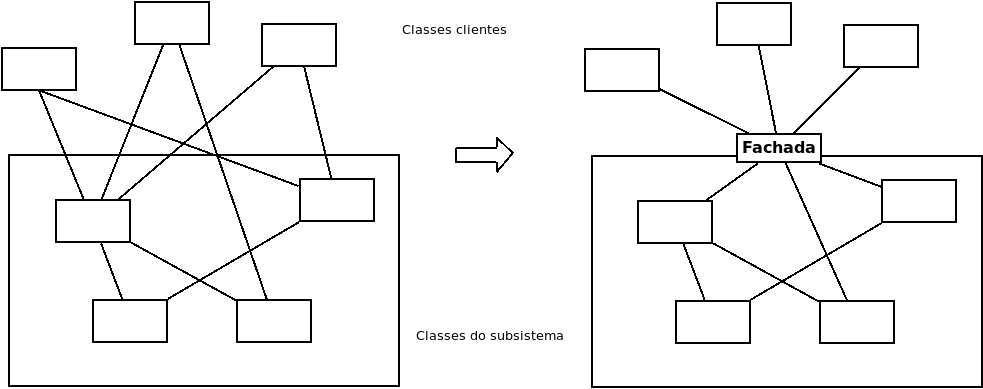
\includegraphics[scale=0.42]{fachada.png}
\caption{Estrutura Genérica do Padrão Fachada}\label{fig:fachada}
\end{center}
\end{figure}

O padrão da Fachada pode ser usado para reduzir o número de objetos com os quais um objeto cliente tem de lidar, além da simplificação da interface.

\subsection{O Padrão Adaptador (\textit{Adapter})}
\subsubsection{Propósito}
Converte a interface de uma classe em uma outra interface esperada pelos clientes. Adaptador permite que classes trabalhem juntas, o que não seria possível por incompatibilidade de interfaces.
 
\subsubsection{Problema}
Um sistema tem os dados e o comportamento corretos, mas a interface errada. Tipicamente usado quando você tem de fazer algo derivado de uma classe abstrata.

\subsubsection{Solução}
O \emph{Adaptador} fornece um embrulho (uma roupagem) com a interface desejada.

\subsubsection{Participantes e colaboradores}
O \emph{Adaptador} adapta a interface de um \emph{Adaptado} para casar com aquela do \emph{Objetivo} do Adaptador (a classe de quem ela deriva). Isto permite ao \emph{Cliente} usar o \emph{Adaptado} como se ele fosse do tipo do \emph{Objetivo}.

\subsubsection{Consequências}
O padrão Adaptador permite o uso de objetos pré-existentes em novas estruturas de classes sem ficar limitado às suas interfaces antigas.

\subsubsection{Implementação}
Contém a classe existente numa outra classe. A nova classe tem a interface requerida e chama os métodos pela classe contida.

\subsubsection{Estrutura Genérica}
A estrutura genérica do Padrão Adaptador é ilustrado na figura \ref{fig:adaptador}.

\begin{figure}[h]
\begin{center}
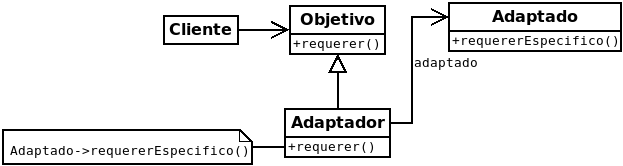
\includegraphics[scale=0.6]{adaptador.png}
\caption{Estrutura Genérica do Padrão Adaptador}\label{fig:adaptador}
\end{center}
\end{figure}

Existem dois tipos de padrões de Adaptadores:
\begin{description}
\item[Padrão Adaptador de Objeto:] O padrão de Adaptador, geralmente, exemplificado é o Adaptador de Objeto que consiste em um objeto adaptador contendo um objeto adaptado.

\item[Padrão Adaptador de Classe:] Um outro modo de implementar o padrão Adaptador é com herança múltipla. Neste caso, temos um padrão Adaptador de Classe.
\end{description}

É comum, projetistas inexperientes não saberem diferenciar os dois padrões: Fachada e Adaptador. \cite{DP:explained} fornecem a seguinte tabela para compará-los:

\begin{table}[h]
\caption{Comparação entre os padrões Fachada e Adaptador}\label{tab:fachadaxadaptador}
\begin{center}
\begin{tabular}{lll}
 & \textbf{Fachada} & \textbf{Adaptador} \\
\hline
Há classes pré-existentes? & Sim & Sim \\
Há uma interface para a qual devemos projetar? & Não & Sim \\
Um objeto precisa ter comportamento polimórfico? & Não & Provavelmente \\
Uma interface mais simples é necessária? & Sim & Não\\
\hline %\hline
\end{tabular}
\legend{Fonte: \cite{DP:explained}}
\end{center}\end{table}

\subsubsection{Exemplo de Adaptador}
A figura \ref{fig:adaptCirc} mostra como uma classe \emph{CirculoEspc} é adaptada para uma classe \emph{Circulo}. Se o código da \emph{CirculoEspc} fosse acessível, ela poderia herdar de \emph{Circulo}, mas, se a classe faz parte de uma biblioteca externa proprietária, não será possível alterar a hierarquia de classes. Outra razão para a classe \emph{CirculoEspc} não ser derivada de \emph{Circulo} é que este tipo de projeto tem alto grau de acoplamento, herança tem alto grau de acoplamento, agregação mantêm um grau de acoplamento menor, tornando o projeto mais flexível para mudanças. 

\begin{figure}[h]
\begin{center}
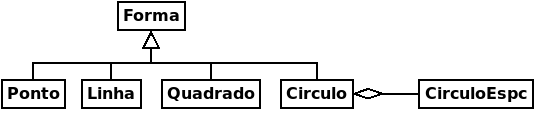
\includegraphics[scale=0.5]{adaptCirc.png}
\caption{Adaptação de CirculoEspc com Circulo}\label{fig:adaptCirc}
\end{center}
\end{figure}


\subsection{O Padrão Fabrica Abstrata (\textit{Abstract Factory})}

O padrão da Fabrica Abstrata é um dos padrões de projeto que procuram abstrair o processo de instanciação. Este tipo de padrão ajuda a tornar um sistema independente de como seus objetos são criados, compostos e representados. Ele esconde como instâncias das classes são criadas e são postas juntas.

\subsubsection{Propósito}
Fornece uma interface para a criação de famílias de objetos relacionados ou dependentes sem especificar as suas classes concretas.

\subsubsection{Problema}
Famílias de objetos relacionados precisam ser instanciadas.

\subsubsection{Solução}
Coordena a criação de famílias de objetos. Fornece uma maneira para retirar as regras de como realizar a instanciação do objeto cliente que está usando estes objetos criados.

\subsubsection{Participantes e Colaboradores}
A FabricaAbstrata define a interface de como criar cada membro da família de objetos requeridos. Tipicamente, cada família é criada usando sua própria FabricaConcreta.

\subsubsection{Consequências}
O padrão isola as regras de quais objetos usar da lógica de como usar estes objetos.

\subsubsection{Implementação}
Defina uma classe abstrata que especifica quais objetos devem ser feitos. Implemente, então, uma classe concreta para cada família.

\subsubsection{Estrutura Genérica}
\begin{figure}[h]
\begin{center}
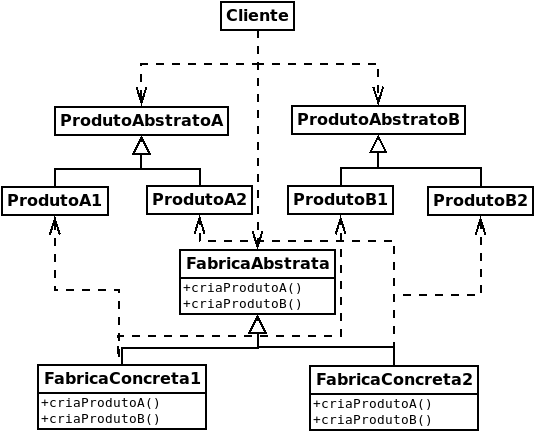
\includegraphics[scale=0.5]{absFact.png}
\caption{Estrutura Genérica do Padrão Fabrica Abstrata}\label{fig:absFab}
\end{center}
\end{figure}

\subsection{O Padrão Método Fabrica (\textit{Factory Method})}
\subsubsection{Propósito}
Define uma interface para a criação de um objeto, mas deixa que uma subclasse decida qual classe instanciar. Adia a instanciação para as subclasses.

\subsubsection{Problema}
Uma classe precisa instanciar uma derivação de uma outra classe, mas não sabe qual. O \emph{Factory Method} permite que uma classe derivada tome a decisão.

\subsubsection{Solução}
Uma classe derivada toma a decisão de qual classe instanciar e como.

\subsubsection{Participantes e colaboradores}
\emph{Produto} é a interface do tipo de ojeto que a \emph{Factory Method} cria. \emph{Creator} é a interface que define a \emph{Factory Method}.

\subsubsection{Consequências}
Clientes precisarão derivar a classe Creator para ter um \emph{ProdutoConcreto}.

\subsubsection{Implementação}
Use um método na classe abstrata que é abstrato. O código da classe abstrata refere-se a este método quando precisa instanciar um objeto contido , mas ainda não sabe qual objeto particular é necessário.

\subsubsection{Estrutura Genérica}

\begin{figure}[h]
\begin{center}
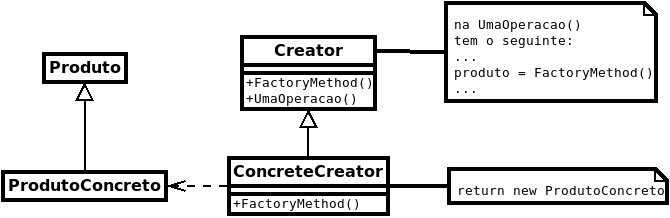
\includegraphics[scale=0.6]{factoryMethod.png}
\caption{Estrutura Genérica do padrão Método Fabrica.}\label{fig:factMeth}
\end{center}
\end{figure}

O padrão Método Fabrica é normalmente usado na definição de \textit{frameworks}. Isto porque frameworks existem num nível abstrato. Geralmente, eles não sabem e não deveriam se preocupar  com a instanciação de objetos específicos. Eles precisam adiar as decisões sobre objetos específicos para usuários de \textit{frameworks}.

\subsection{O Padrão Observador (\textit{Observer})}
\subsubsection{Propósito}
\subsubsection{Problema}
\subsubsection{Solução}
\subsubsection{Participantes e colaboradores}
\subsubsection{Consequências}
\subsubsection{Implementação}
\subsubsection{Estrutura Genérica}

\subsection{O Padrão Composição (\textit{Composite})}
\subsubsection{Propósito}
\subsubsection{Problema}
\subsubsection{Solução}
\subsubsection{Participantes e colaboradores}
\subsubsection{Consequências}
\subsubsection{Implementação}
\subsubsection{Estrutura Genérica}

\subsection{O Padrão Iterador (\textit{Iterator})}
\subsubsection{Propósito}
\subsubsection{Problema}
\subsubsection{Solução}
\subsubsection{Participantes e colaboradores}
\subsubsection{Consequências}
\subsubsection{Implementação}
\subsubsection{Estrutura Genérica}

\subsection{O Padrão Visitante (\textit{Visitor})}
\subsubsection{Propósito}
\subsubsection{Problema}
\subsubsection{Solução}
\subsubsection{Participantes e colaboradores}
\subsubsection{Consequências}
\subsubsection{Implementação}
\subsubsection{Estrutura Genérica}

\subsection{O Padrão Estratégia (\textit{Strategy})}
\subsubsection{Propósito}
Permite que você use regras de negócios ou algoritmos diferentes dependendo do contexto nos quais eles ocorrem.

\subsubsection{Problema}
A seleção de um algoritmo que precisa ser aplicado depende do cliente que faz a chamada ou dos dados sobre os quais ele age. Se você só tiver uma regra que não muda, você não precisa do padrão Estratégia.

\subsubsection{Solução}
Separa a seleção do algoritmo da implementação do algoritmo. Permite que a seleção seja feita baseada no contexto.

\subsubsection{Participantes e colaboradores}
\emph{Estratégia} especifica como os diferentes algoritmos são usados. \emph{EstratégiasConcretas} implementa estes diferentes algoritmos. \emph{Contexto} usa uma \emph{EstratégiaConcreta} especifica com uma referência do tipo \emph{Estratégia}. Estratégia e Contexto interagem para implementar o algoritmo escolhido. (As vezes, \emph{Estratégia} deve pedir \emph{Contexto}.) O \emph{Contexto} direciona pedidos dos seus clientes para \emph{Estratégia}.

\subsubsection{Consequências}
O padrão Estratégia define uma família de algoritmos. O uso de condicionais e switches (casos) podem ser eliminados. Você pode invocar todos os algoritmos do mesmo jeito. (Eles devem todos ter a mesma interface.) A interação entre \emph{EstratégiasConcretas} e \emph{Contexto} pode requerer a adição de métodos que obtêm o estado do \emph{Contexto}.

\subsubsection{Implementação}
\subsubsection{Estrutura Genérica}

\subsection{O Padrão Decorador (\textit{Decorator})}
\subsubsection{Propósito}
\subsubsection{Problema}
\subsubsection{Solução}
\subsubsection{Participantes e colaboradores}
\subsubsection{Consequências}
\subsubsection{Implementação}
\subsubsection{Estrutura Genérica}

\subsection{O Padrão Método Gabarito (\textit{Template Method})}
\subsubsection{Propósito}
\subsubsection{Problema}
\subsubsection{Solução}
\subsubsection{Participantes e colaboradores}
\subsubsection{Consequências}
\subsubsection{Implementação}
\subsubsection{Estrutura Genérica}

\subsection{O Padrão \textit{Singleton}}
\subsubsection{Propósito}
\subsubsection{Problema}
\subsubsection{Solução}
\subsubsection{Participantes e colaboradores}
\subsubsection{Consequências}
\subsubsection{Implementação}
\subsubsection{Estrutura Genérica}

\subsection{O Padrão Trava Duplamente Verificada (\textit{Lock Double Checked})}
\subsubsection{Propósito}
\subsubsection{Problema}
\subsubsection{Solução}
\subsubsection{Participantes e colaboradores}
\subsubsection{Consequências}
\subsubsection{Implementação}
\subsubsection{Estrutura Genérica}

\subsection{O Padrão Ponte (\textit{Bridge})}
\subsubsection{Propósito}
\subsubsection{Problema}
\subsubsection{Solução}
\subsubsection{Participantes e colaboradores}
\subsubsection{Consequências}
\subsubsection{Implementação}
\subsubsection{Estrutura Genérica}

\subsection{O Padrão Construtor (\textit{Builder})}
\subsubsection{Propósito}
\subsubsection{Problema}
\subsubsection{Solução}
\subsubsection{Participantes e colaboradores}
\subsubsection{Consequências}
\subsubsection{Implementação}
\subsubsection{Estrutura Genérica}

\subsection{O Padrão Protótipo (\textit{Prototype})}
\subsubsection{Propósito}
\subsubsection{Problema}
\subsubsection{Solução}
\subsubsection{Participantes e colaboradores}
\subsubsection{Consequências}
\subsubsection{Implementação}
\subsubsection{Estrutura Genérica}

\subsection{O Padrão Piscina de Objetos (\textit{Object Pool})}
\subsubsection{Propósito}
\subsubsection{Problema}
\subsubsection{Solução}
\subsubsection{Participantes e colaboradores}
\subsubsection{Consequências}
\subsubsection{Implementação}
\subsubsection{Estrutura Genérica}

\subsection{O Padrão Cadeia de Responsabilidade (\textit{Chain of Responsability})}
\subsubsection{Propósito}
\subsubsection{Problema}
\subsubsection{Solução}
\subsubsection{Participantes e colaboradores}
\subsubsection{Consequências}
\subsubsection{Implementação}
\subsubsection{Estrutura Genérica}

\subsection{O Padrão Comando (\textit{Command})}
\subsubsection{Propósito}
\subsubsection{Problema}
\subsubsection{Solução}
\subsubsection{Participantes e colaboradores}
\subsubsection{Consequências}
\subsubsection{Implementação}
\subsubsection{Estrutura Genérica}

\subsection{O Padrão Peso Pena (\textit{Flyweight})}
\subsubsection{Propósito}
\subsubsection{Problema}
\subsubsection{Solução}
\subsubsection{Participantes e colaboradores}
\subsubsection{Consequências}
\subsubsection{Implementação}
\subsubsection{Estrutura Genérica}

\subsection{O Padrão Interpretador (\textit{Interpreter})}
\subsubsection{Propósito}
\subsubsection{Problema}
\subsubsection{Solução}
\subsubsection{Participantes e colaboradores}
\subsubsection{Consequências}
\subsubsection{Implementação}
\subsubsection{Estrutura Genérica}

\subsection{O Padrão Mediador (\textit{Mediator})}
\subsubsection{Propósito}
\subsubsection{Problema}
\subsubsection{Solução}
\subsubsection{Participantes e colaboradores}
\subsubsection{Consequências}
\subsubsection{Implementação}
\subsubsection{Estrutura Genérica}

\subsection{O Padrão \textit{Memento}}
\subsubsection{Propósito}
\subsubsection{Problema}
\subsubsection{Solução}
\subsubsection{Participantes e colaboradores}
\subsubsection{Consequências}
\subsubsection{Implementação}
\subsubsection{Estrutura Genérica}

\subsection{O Padrão \textit{Proxy}}
\subsubsection{Propósito}
\subsubsection{Problema}
\subsubsection{Solução}
\subsubsection{Participantes e colaboradores}
\subsubsection{Consequências}
\subsubsection{Implementação}
\subsubsection{Estrutura Genérica}

\subsection{O Padrão Estado (\textit{State})}
\subsubsection{Propósito}
\subsubsection{Problema}
\subsubsection{Solução}
\subsubsection{Participantes e colaboradores}
\subsubsection{Consequências}
\subsubsection{Implementação}
\subsubsection{Estrutura Genérica}

\section{O Processo de Pensar em Padrões}

De acordo com \citeonline{design:patterns}, o processo de pensar em padrões segue os passos:
\begin{enumerate}
\item \textbf{Identifique os padrões:} Encontre os padrões no domínio do problema;
\item \textbf{Analise e aplique os padrões:} Para o conjunto de padrões a ser analisado, realize os passos a) até d):
\begin{enumerate}
\item \textbf{Ordene os padrões pelo contexto de criação:} Ordene os padrões de acordo com como eles criam contexto para cada um dos outros padrões. A ideia é a de que um padrão vai criar contexto para um outro, não que dois padrões vão criar contexto um para o outro.
\item \textbf{Selecione cada padrão e expanda o projeto:} Usando sua ordenação, selecione o próximo padrão da lista e use-o para um projeto conceitual de alto nível.
\item \textbf{Identifique padrões adicionais:} Identifique qualquer padrão adicional que surja durante a sua análise. Adicione-o ao conjunto de padrões a serem analisados.
\item \textbf{Repita:} Repita para o conjunto de padrões que ainda não foram integrados ao projeto conceitual.
\end{enumerate}
\item \textbf{Adicione detalhes:} Adicione os detalhes a medida que se tornarem necessários ao projeto. Expanda as definições das classes e dos métodos.
\end{enumerate}

\cite{DP:explained} dizem que para aplicar os padrões aos seus projetos é necessário que conheça bem o domínio do problema. Além disso, pensar em padrões nem sempre é aplicável, mas análise de comunalidade e variabilidade é geralmente mais usável. Os autores mostram como aplicar os passos no projeto de um CAD/CAM.
